\documentclass[a4paper]{article}

\usepackage[]{amsmath} 
\usepackage[]{amssymb} 
\usepackage[]{amsthm} 

\usepackage[]{microtype} 
\usepackage[]{mathtools} 
\usepackage[]{minted} 

\usepackage[]{graphicx} 
\graphicspath{{./pictures/}}

\usepackage[]{hyperref} 
\usepackage[]{cleveref} 

\mathtoolset{\centercolon}

\title{\textsc{Assignment 1 \\ MATINF4170 \\ Spline methods}}
\author{Ivar Haugal{\o}kken Stangeby}

\begin{document}
    \maketitle

    \begin{abstract}
       In this assignment we discuss two methods for curve generation,
       Neville-Aitken for interpolating curves, and de Casteljau for B\'ezier
       curves. We also prove that B-splines has compact support, given
       explicitly by the degree of the B-spline. Finally we use the recursive
       definition of B-splines of degree $p$ to evaluate a specific B-spline.
    \end{abstract} 

    \section*{Exercise 1.3}
    \label{sec:exercise_1_3}
    
    In this exercise we take a look at the Neville-Aitken algorithm for
    evaluating points on an interpolating curve. In the general setup we are
    given $p+1$ control points, $\left\{ c_j \right\}_{j=0}^p$, as well as
    $p+1$ strictly increasing parameter values $\left\{ t_j \right\}_{j=0}^p$.
    The integer $p$ ends up being the degree of the interpolating polynomial.
    The algorithm was implemented in \textsc{Python} and the source code is
    given in \Cref{lst:nev_ait}.  We wish to interpolate $N$ points on the
    semicircle $\mathcal{C} \coloneqq \left\{ \left( \cos(t), \sin(t) \right)
    \mid t \in [0, \pi]\right\}$ and study the effect of varying the number of
    interpolation points $N$, as well as the effect of varying the parameter
    values. 
   
    We chose two distinct parametrizations, one being the uniform
    parametrization given by
    \begin{equation}
        \notag
        t_{j+1} - t_j = 1
    \end{equation}
    for $j = 0, \ldots, N-1$ and with $t_0 = 0$. The other one being tailored
    to misbehave for increasing $N$ was generated using a cumulative sum of
    random numbers, that is:
    \begin{equation}
        \notag
        t_{j+1} - t_j = r_j
    \end{equation}
    where $r_j$ is a random integer in $\mathbb{Z}_5$ and $t_0 = 0$.  The
    uniform parametrization behaved quite nicely under increasing $N$, as can
    be seen in \Cref{fig:uniform}.  The random parametrization on the other
    hand was very unstable under increasing $N$ and hence yields a very bad
    interpolation to the semi circle for large $N$, as seen in \Cref{fig:random}.

    \begin{figure}[htbp]
        \centering
        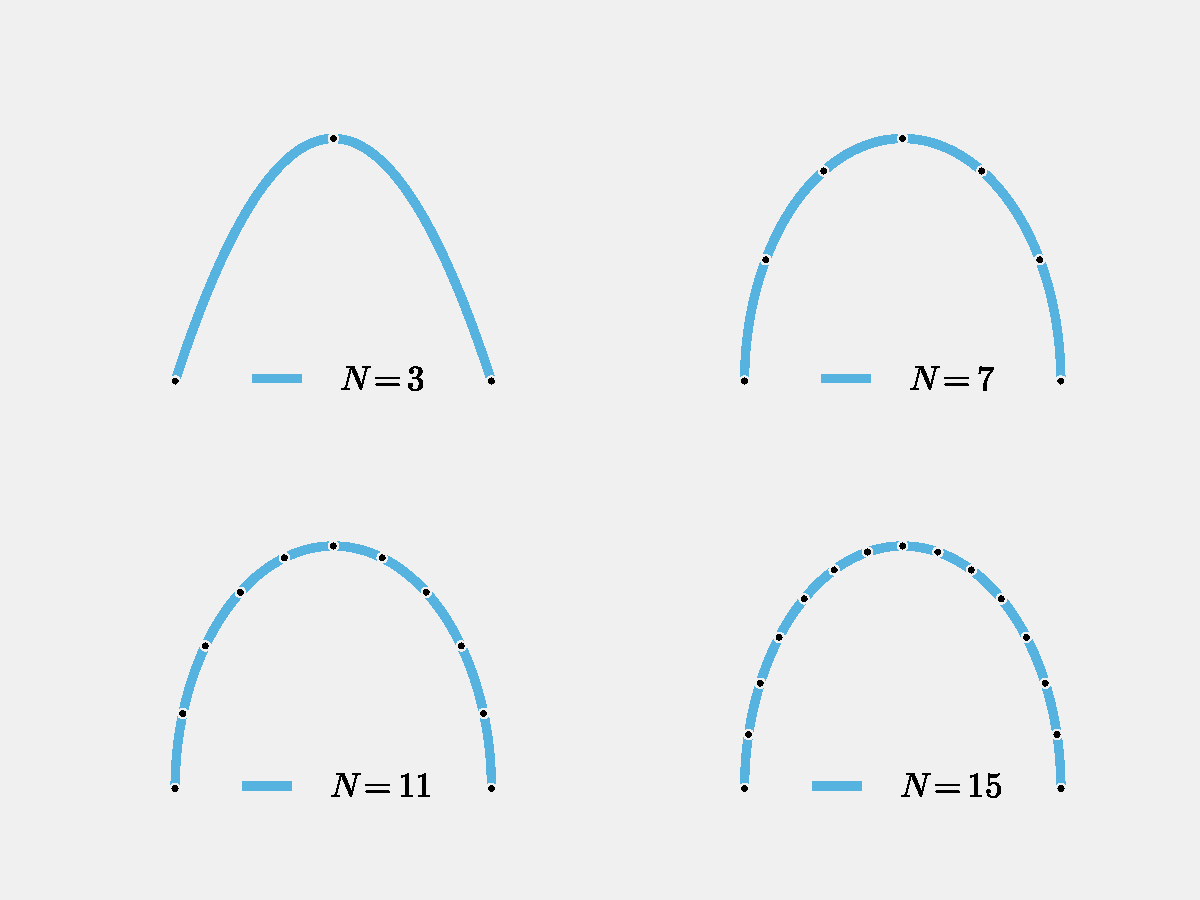
\includegraphics[width=0.8\linewidth]{uniform.pdf}
        \caption{Uniform parametrization of the parameter values, i.e.,
    \begin{equation}
        \notag
        \left\{ t_j \right\}_{j=0}^{N-1} = \left\{ 0, 1, \ldots, N-1 \right\}.
    \end{equation}
    As $N$ increases, we see that the interpolating polynomial converges fairly
quickly to the unit semi circle. The uniform parametrization yields a good
interpolation.}
        \label{fig:uniform}
    \end{figure}
    
    \begin{figure}[htpb]
        \centering
        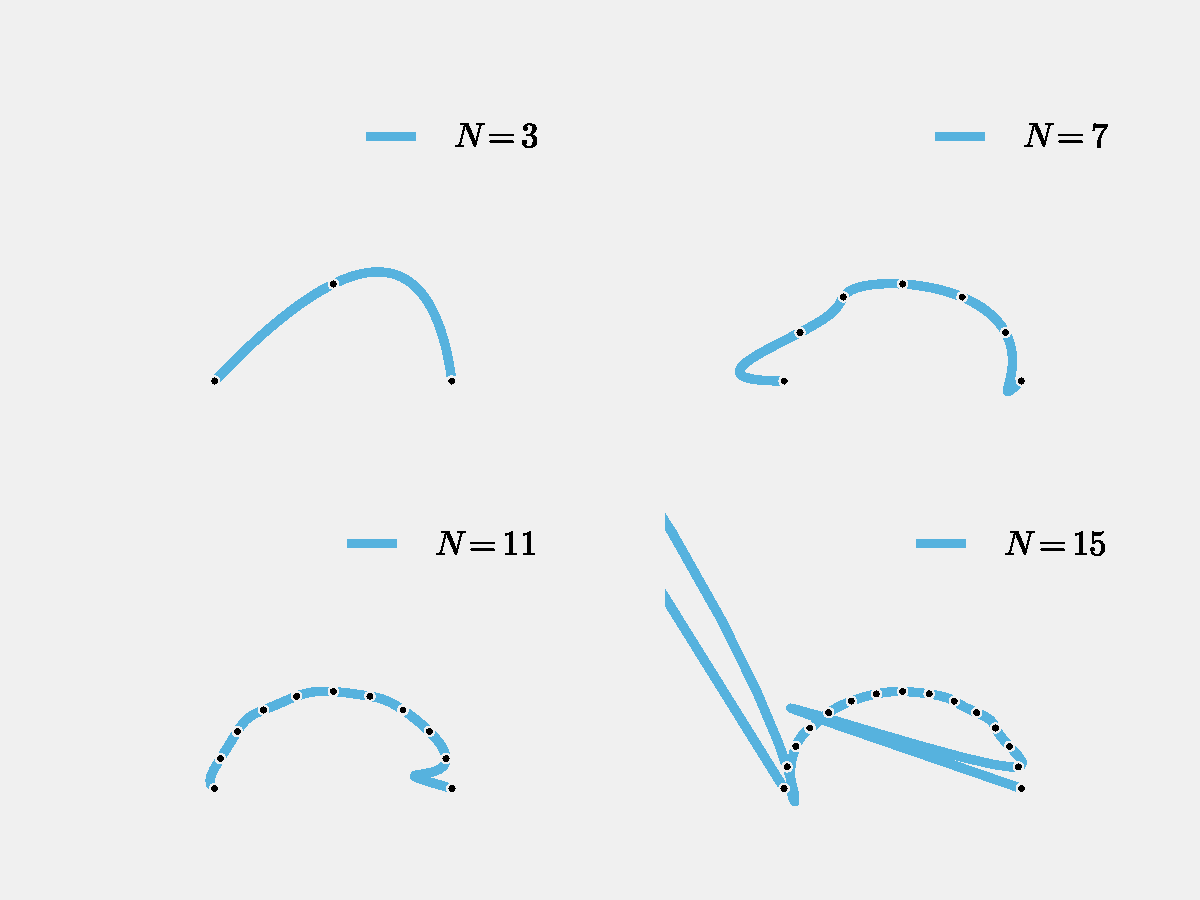
\includegraphics[width=0.8\linewidth]{random.pdf}
        \caption{This parametrization was generated using a random generator.
            The parameter values for $N = 15$ ended up being
            $$\left\{t_j\right\}_{0}^{14} = \left\{2, 4,  5,  6,
            8, 10, 12, 14, 16, 17, 18, 20, 21, 23, 25\right\},$$ and for lower $N$ a
        subsequence of this was used.}
        \label{fig:random}
    \end{figure}

    \begin{listing}
    \begin{minted}{python}
def NevAit(T, c_points, t_points, eps=1.0E-14):
    """
    The Neville Aitkens Given p + 1 control points c_points and p+1
    strictly increasing parameter values t_points, computes the polynomial
    curve of degree p that interpolates the control points.
    """
    t = t_points
    c = np.array(c_points, dtype=np.float64)
    p = len(c) - 1
    for k in range(1, p + 1):
        for j in range(0, p - k + 1):
            denum = (t[j+k] - t[j]) 
            if abs(denum) <= eps:
                c[j] = 0
                continue
            l_one = (t[j+k] - T) / denum
            l_two = (T - t[j]) / denum
            c[j] = l_one*c[j] + l_two * c[j+1]
    return c[0]
    \end{minted}
    \caption{The Neville-Aitken algorithm implemented in \textsc{Python}. The
        algorithm uses in-place replacement of the newly computed values in
        order to save memory, as well as time. No other numerical optimizations
    has been made.}
    \label{lst:nev_ait}
    \end{listing}

    \section*{Exercise 1.4}
    \label{sec:exercise_1_4}
    
    In this exercise we look at the de Casteljau algorithm for computing points
    on a B\'ezier curve. It is very similar to the Neville-Aitken algorithm,
    however there is one big difference.  While the Neville-Aitken algorithm
    parametrizes on adjacent parameter intervals, yielding convex combinations
    only in the last step of the algorithm, the de Casteljau algorithm
    parametrizes each line segment over the same interval. This has the added
    benefit of convex combinations in every step of the algorithm and yields
    higher numerical stability. Due to this, the resulting curve interpolates
    only the first and the last control point, hence the interpolatory nature
    of the Neville-Aitken is lost. The algorithm was implemented in \textsc{Python}
    and the code can be seen in \Cref{lst:decasteljau}.

    Using the same data as in the previous exercise the resulting curve can be
    seen in \Cref{fig:bezier}. As we can see the interpolation property has
    been lost for the interior control points.

    \begin{listing}
        \begin{minted}{python}
def deCasteljau(T, c_points, interval_start=0, interval_stop=1):
    """
    The de Casteljau algorithm.
    Given p + 1 control points c_points, computes the point on the bezier curve
    at parameter value T.
    """
    T = (interval_stop - T) / float(interval_stop - interval_start)
    c = np.array(c_points, dtype=np.float64)
    p = len(c_points) - 1

    for k in range(1, p+1):
        for j in range(0, p - k + 1):
            c[j] = (1-T)*c[j] + T * c[j+1]

    return c[0]
        \end{minted} 
        \caption{The de Casteljau algorithm for computing points on a B\'ezier
        curve. Again, the implementation uses in place replacement of newly
    computed values. No other numerical optimizations has been made.}
        \label{lst:decasteljau}
    \end{listing}

    \begin{figure}[htpb]
        \centering
        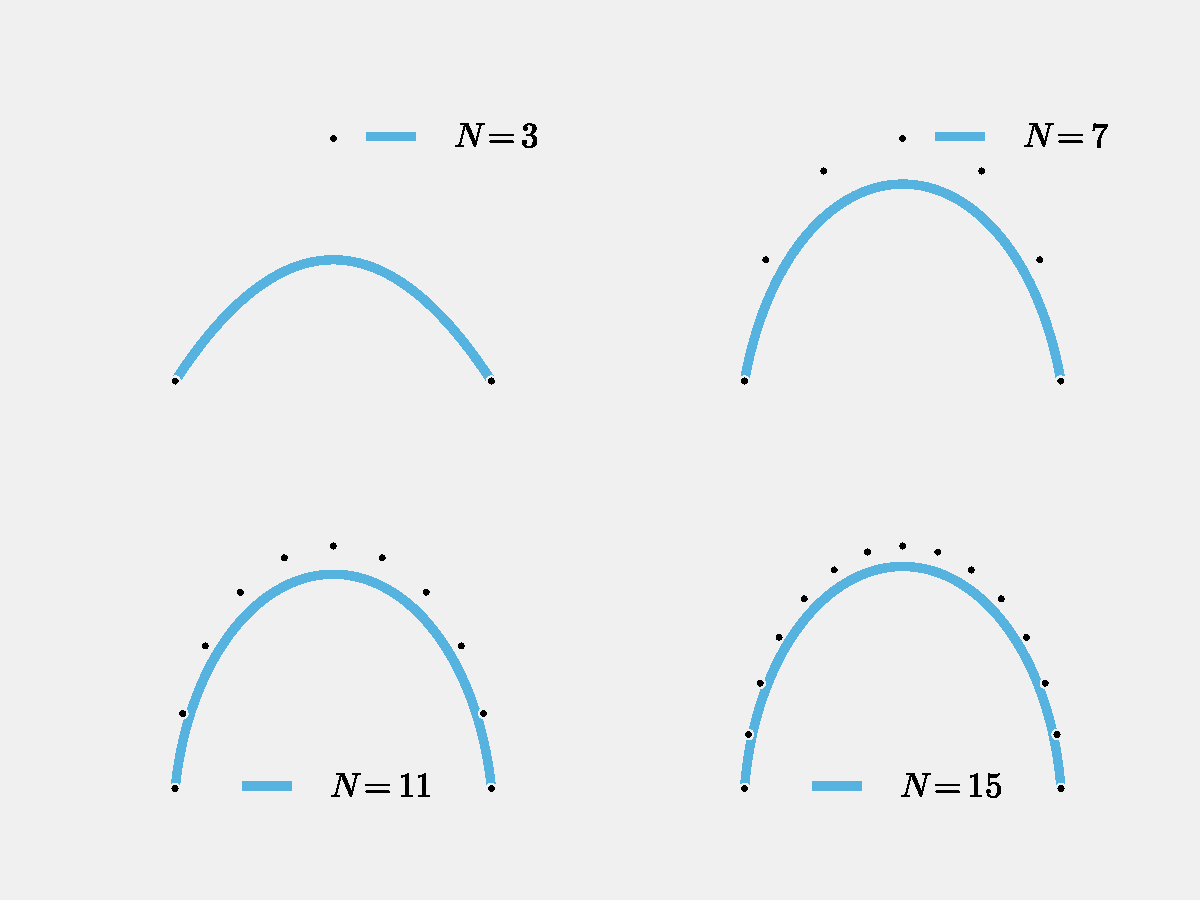
\includegraphics[width=0.8\linewidth]{bezier.pdf}
        \caption{Computing convex combinations of the line segments yields what
            we call a B\'ezier curve. The curve has nice geometric properties
            due to it always lying in the convex hull of its control points. It
            therefore resembles the control polygon nicely. It does however not
            interpolate the interior control points.}
        \label{fig:bezier}
    \end{figure}

    \section*{Exercise 1.7}
    \label{sec:exercise_1_7}
    
    We wish to show that the $j$th B-spline of degree $p$, $B_{j, p}$ only
    relies on the knots $t_j, \ldots, t_{j+p+1}$. In addition we want to show
    that $B_{j, p}$ vanishes outside these knots.  We first recall that $B_{j,
    0}$ is defined as
    \begin{equation}
        \label{eq:def}
        B_{j, 0}(t) = \begin{cases}
            1, & t_j \leq t < t_{j+1};\\
            0,
        \end{cases}
    \end{equation}
    and that $B_{j, p}$ is defined recursively as
    \begin{equation}
        \label{eq:rec}
        B_{j, p}(t) = \frac{t - t_j}{t_{j+k} - t_j}B_{j, p-1}(t) + \frac{t_{j+1+k} - t}{t_{j+k+1} - t_{j+1}} B_{j+1, k-1}(t).
    \end{equation}

    We apply strong induction on $p$. The base case with $p = 0$ follows
    immediately from the definition given in \Cref{eq:def}. Assume inductively
    that the hypothesis holds for $p = 0, 1, \ldots, k - 1$. We wish to show
    that it must then also hold for $p = k$. However, since the two lower
    degree B-splines depend only on the knots $t_j, \ldots, t_{j+k-1}$ and
    $t_{j + 1}, \ldots, t_{j+k}$, and we only introduce the new knot
    $t_{j+k+1}$ in the recurrence relation, the claim holds. This closes the
    induction.
    
    To show that $B_{j, p}$ vanishes outside of the knot interval discussed
    above, we first discuss the case where $t < t_j$ and in this case $B_{j,0}
    = 0$. In addition, since the knots are assumed to be increasing $t_j \leq
    t_{j+1}$, we also have that $B_{k, 0} = 0$ for all $k > j$. Consequently,
    all terms in the recurrence relation given in \Cref{eq:rec} are zero, hence
    $B_{j, p} = 0$.  Assume now that $t > t_{j+p+1}$, by the same argument
    above, $B_{k, 0}$ are zero for all $k < j + p + 1$. Hence $B_{j, p} = 0$.

    This result gives us a computational advantage, as for any given parameter
    value $t$, we only need to evaluate the B-splines that are ``active'' on
    the respective knot intervals. This is illustrated in
    \Cref{fig:activesplines}.

    \begin{figure}[htpb]
        \centering
        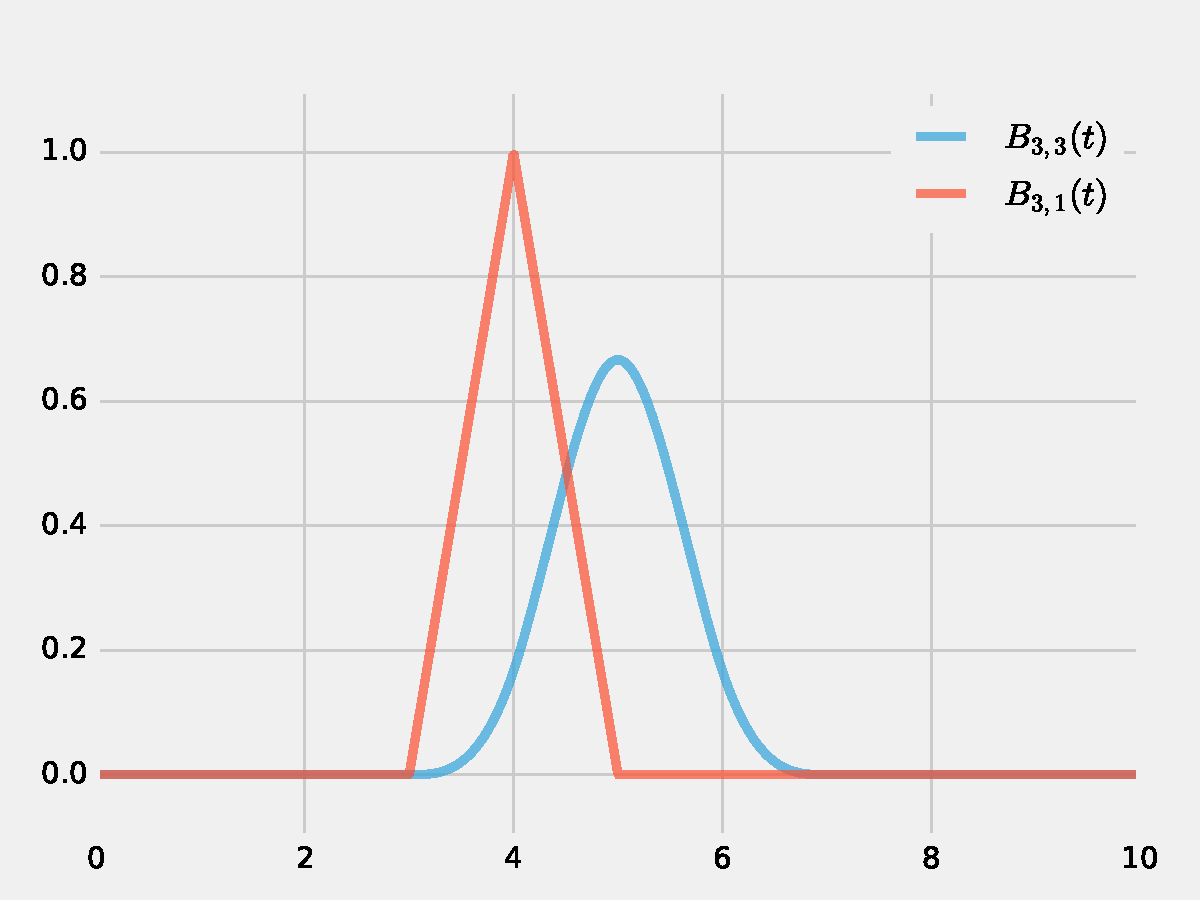
\includegraphics[width=0.8\linewidth]{bsplines.pdf}
        \caption{The third B-splines of degree three and one respectively. The
        knots are uniform. Here we clearly see the support of the basis
    splines, and how each B-spline has a set of knots where it is non-zero.}
        \label{fig:activesplines}
    \end{figure}

    \section*{Exercise 2.1}
    \label{sec:exercise_2_1}
    
    We wish to evaluate the B-spline $B[0, 3, 4, 6](x)$. We first recall that
    for notational purposes, we often write
    \begin{equation}
        \notag
        B_{j, p} = B[t_j, \ldots, t_{j+p+1}]
    \end{equation}
    if the knots have to be emphasized. Using \Cref{eq:rec} we compute
    directly:
    \begin{align*}
        B[0, 3, 4, 6](x) &= \frac{x}{4}B[0, 3, 4](x) + \frac{6-x}{3}B[3, 4, 6](x) \\
                         &= \frac{x}{4}\left( \frac{x}{3} B[0, 3](x) + \frac{x(4-x)}{4}B[3, 4](x) \right)
        + \frac{(6 - x)}{3}\left((x-3)B[3, 4](x) + \frac{(6-x)}{2}B[4, 6](x) \right) \\
                          &= \frac{1}{12}x^2B[0, 3](x) + \frac{1}{12}(-7x^2 + 48x - 72)B[3, 4](x) + \frac{1}{6}(6-x)^2B[4, 6](x).
    \end{align*}
\end{document}
